\documentclass[a4paper]{article}

\usepackage{amsmath}
\usepackage{amssymb}
\usepackage{parskip}    % skip line
\usepackage{biblatex}   % references
\usepackage[hang]{subfigure}
\usepackage[noend]{algpseudocode}
\usepackage{algorithm}

\usepackage{lpi}

% Se scritta in italiano:
%\usepackage[italian]{babel}

\addbibresource{./references.bib}
\graphicspath{ {./media} } % sections/images

\title{%
    Trimap Matting \\
    \phantom{} \\
    \large Scuola d'Arti e Mestieri di Trevano (SAMT) \\
    \large Documentation
}

\author{Paolo Bettelini}

\date{}

\lpisetup%
    {Trimap Matting}

\makenoidxglossaries

\newglossaryentry{FFI}
{
    name=FFI,
    description={Foreign Function Interface}
}

\newglossaryentry{trait}
{
    name=trait,
    description={A trait in Rust defined shared behavior among structures}
}

\begin{document}

\maketitle

\pagebreak

\tableofcontents

\pagebreak

\section{Introduction}

\subsection{Abstract}

\subsection{Information}

This is a project of the Scuola Arti e Mestieri di Trevano (SAMT) under the following circumstances

\begin{itemize}
    \item \textbf{Section}: Computer Science
    \item \textbf{Year:} Fourth
    \item \textbf{Class:} Progetti Individuali
    \item \textbf{Supervisor:} Geo Petrini
    \item \textbf{Title:} Trimap Matting
    \item \textbf{Start date}: 2022-09-29
    \item \textbf{Deadline}: 2022-12-07
\end{itemize}

and the following requirements

\begin{itemize}
    \item \textbf{Documentation}: a full documentation of the work done
    \item \textbf{Diary}: constant changelog for each working session
    \item \textbf{Source code}: source code of the project
\end{itemize}

All the source code and documents can be found at
\href{https://github.com/paolobettelini/trimap-matting}
{https://github.com/paolobettelini/trimap-matting}
\cite{gitrepo}.

\pagebreak

\section{Requirements}

\requirement{00}{CLI tool}{1}{1.1}{none}{
    A CLI tool to execute background removal must be developed
}{
    \subreq{00}{0}{The target image must be specified}
    \subreq{00}{1}{The trimap image can be specified}
    \subreq{00}{2}{The soft mask can be specified}
    \subreq{00}{3}{Either the soft mask or the trimap must be specified}
    \subreq{00}{4}{The program can save the generated background mask}
    \subreq{00}{5}{The program can remove the background and replace it with an image}
    \subreq{00}{6}{The program can remove the background and fill it with a color}
    \subreq{00}{7}{The program can remove the background and leave it transparent}
}

\requirement{01}{Image formats}{1}{1.0}{none}{
    Multiple image formats must be supported
}{
    \subreq{00}{0}{The JPG format must be supported}
    \subreq{00}{1}{The PNG format must be supported}
    \subreq{00}{2}{The WebP format must be supported}
}

\requirement{02}{Size check}{1}{1.0}{none}{
    The executable must assert that the target image and trimap are of the same size
}{%
}

\requirement{03}{GUI}{1}{1.0}{none}{
    A GUI application must be developed in other to interact with the program features
}{%
}

\pagebreak

\section{CLI}

\subsection{Compilation}

The executable can be compiled using the \texttt{cargo}
package manager.

\begin{lstlisting}[style=boxed]
    $ cd matting-cli
    $ cargo build --release
\end{lstlisting}

This will generate an executable (\texttt{matting-cli})
in \texttt{./target/debug}.
In order to make this executable globally available
we can move it into a folder in the \textsc{\$PATH} enviroment
variable, such as \texttt{/usr/bin}.
We may also modify the executable file name to change its invokation
name.

\begin{lstlisting}[style=boxed]
    $ sudo mv target/release/matting-cli /usr/bin/
\end{lstlisting}

We executable can now be invoked by just writing
\begin{lstlisting}[style=boxed]
    $ matting-cli
\end{lstlisting}

\subsection{Usage}

The followings shows the output of the command upon
setting the \texttt{--help} or \texttt{-h} flag.
\begin{lstlisting}[style=boxed]
Matting CLI

Usage: matting-cli [OPTIONS] --target <TARGET>
                   <--mask <MASK>|--trimap <TRIMAP>>

Options:
  -i, --target <TARGET>        Target image
      --mask <MASK>            Background mask image
      --trimap <TRIMAP>        Trimap image
      --save-mask <SAVE_MASK>  Save mask path
  -o, --output <OUTPUT>        Output image
  -f, --fill <FILL>            Fill background action
  -t, --transparent            Transparent background action
  -r, --replace <REPLACE>      Replace background action
      --verbose                Verbose flag
  -h, --help                   Print help information
  -V, --version                Print version information
\end{lstlisting}

The \texttt{--target} parameter specifies the image
on which the operation needs to be applied.
This parameter is \underline{mandatory}.

The \texttt{--trimap} parameter specifies the trimap
image which will be used to generate the alpha mattes.

The \texttt{--mask} parameter specifies the image
containing the alpha mattes to use.

The parameter \texttt{--trimap} and \texttt{--mask}
are mutually exclusive and one of them is \underline{mandatory}.

The advantage of using \texttt{--mask} over
\texttt{--trimap} is that the alpha mattes are
already given rather than having to be computed.
This can save lots of computational times.
The alpha mattes image can be saved on the file system
by specifying the \texttt{--save-mask} parameter.

There are 3 different operations that can be applied
to the background of the result: \texttt{--transparent},
\texttt{--replace} or \texttt{--fill}.
These operations are mutually exclusive and if one is specified,
the \texttt{--output} parameter can be set to
specify the path where the resulting image will be saved.
If the \texttt{--output} parameter is not specified then it will produce
a file name with the current timestmap.

\textbf{Note:} the argument of \texttt{--color} can be any valid
CSS color. See \cite{csscolors} for the documentation.

The \texttt{--verbose} flag is optional and will print additional
information about what the program is doing and the elapsed
time of each operation.

\subsection{Examples}

The following command generates a mask of the alpha mattes
given a trimap and saves it to \texttt{mask.png}.
\begin{lstlisting}[style=boxed]
    $ matting-cli -i target.jpg --trimap trimap.png
        --save-mask mask.png
\end{lstlisting}

The following command removes the background of an image
given its mask.
\begin{lstlisting}[style=boxed]
    $ matting-cli -i target.jpg --mask mask.png
        -o out.png --transparent
\end{lstlisting}

The following command removes the background of an image
given its mask and replaces it with the color \texttt{\#A3BF13}.
\begin{lstlisting}[style=boxed]
    $ matting-cli -i target.jpg --mask mask.png
        -o out.png --fill "#A3BF13"
\end{lstlisting}

The following command removes the background of an image
given its mask and replaces it with the image \texttt{background.png}.
\begin{lstlisting}[style=boxed]
    $ matting-cli -i target.jpg --mask mask.png
        -o out.png --replace background.png
\end{lstlisting}

The following shows the output of the program when the \texttt{--verbose}
flag is set. This command computes the alpha mattes given a trimap,
then it saves the generated mask, fills the background of the image
with the color red and then saves the result.
\begin{lstlisting}[style=boxed]
    $ matting-cli -i target.jpg --trimap trimap.png
        --save-mask mask.png -o out.png --fill red --verbose
    
    Reading target image... Done! [4.021485ms]
    Reading trimap image... Done! [1.976477ms]
    Generating soft mask... Done! [7.104532642s]
    Reading target image... Done! [178.884124ms]
    Saving soft mask... Done! [509.050896ms]
    Filling background with color... Done! [117.90393ms]
    Saving output... Done! [954.085622ms]
\end{lstlisting}

\pagebreak

\section{Trimap Matting}
\label{sec:trimat}


Matting is a technique used to extract an object
from an image.
Trimap matting is a term used to refer to the process
of generating alpha mattes\cite{matte} for an object
% https://en.wikipedia.org/wiki/Matte_(filmmaking)
in an image given an initial
approximation of its borders.

The goal of this process is to determine
how much each pixel of a target image is part of the
object that needs to be extracted.
This means that given a pixel \(P_{x,y}\)
we want to find a value \(\alpha \in \mathbb{R}\) such that
\[
    P_{x,y} = \alpha F_{x,y} + (1-\alpha) B_{x,y},
    \quad \alpha \in [0;1]
\]
where \(F\) represents the foreground color
and \(B\) represents the background color at a given pixel.

Note that the multiplicative operator here is the scalar vector multiplication.
This is because the pixels are represented by a vector of values,
usually \({\mathbb{R}}^3\) or \({\mathbb{R}}^4\) (for transparent images).

The trimap is an approximation of the alpha mattes.
The black dye represents background-only space, the white dye
represents foreground-only space whilst the gray one
delimits the distinction between the two.

Here are some examples using an image of a plant.

\begin{figure}[h]
    \begin{minipage}{0.33\textwidth}
        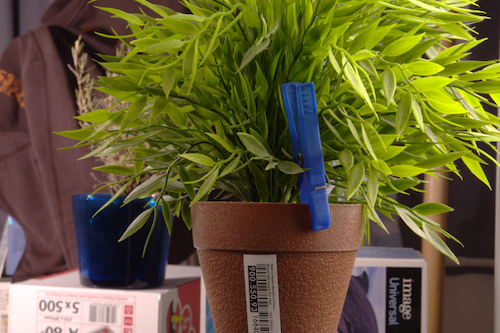
\includegraphics[width=\textwidth]{target.jpg}
        \caption{Plant Image}
    \end{minipage}
    \begin{minipage}{0.33\textwidth}
        
\includegraphics[width=\textwidth]{trimap.png}
        \caption{Plant Trimap}
    \end{minipage}
    \begin{minipage}{0.33\textwidth}
        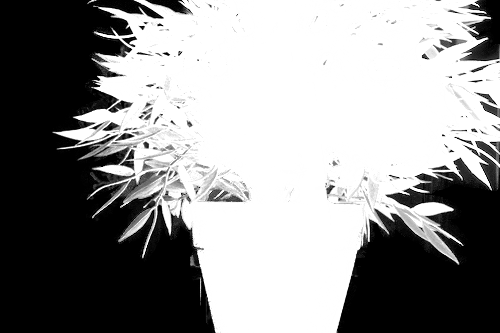
\includegraphics[width=\textwidth]{mask.png}
        \caption{Plant Soft Mask}
    \end{minipage}
\end{figure}

Once the alpha mattes are generated (soft mask) we can use them
to extract the object from the target image.
Thus, we can remove the background behind the object,
fill the background with a color, replace it with another image
or leave it transparent.

Given a target image with pixels \(T_{x,y}\), the alpha
mattes \(\alpha_{x,y}\) and the pixels of the replacement image
\(R_{x,y}\) we can compute the pixels of the output image \(T_{x,y}'\)
as follows
\[
    T_{x,y}' = 
    \alpha_{x,y} \cdot T_{x,y} + (1 - \alpha_{x,y}) \cdot R_{x,y}
\]
If we want to replace the background with a color we can consider.
\(R={(r,g,b)}^t\) \\
If we just want to leave the background transparent, meaning
\(T' \in {\mathbb{R}}^4\), we have
\[
    T_{x,y}' = 
    \alpha_{x,y} \cdot T_{x,y}
\]
and the alpha value for \(T_{x,y}\) is set to \(\alpha_{x,y}\).

\begin{figure}[h]
    \begin{minipage}{0.33\textwidth}
        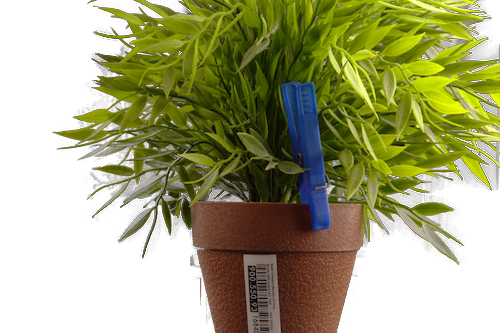
\includegraphics[width=\textwidth]{result3.png}
        \caption{Transparency}
    \end{minipage}
    \begin{minipage}{0.33\textwidth}
        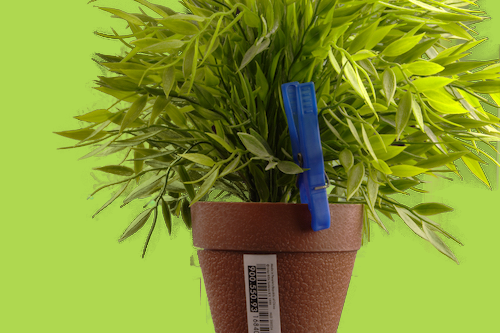
\includegraphics[width=\textwidth]{result2.png}
        \caption{Color fill}
    \end{minipage}
    \begin{minipage}{0.33\textwidth}
        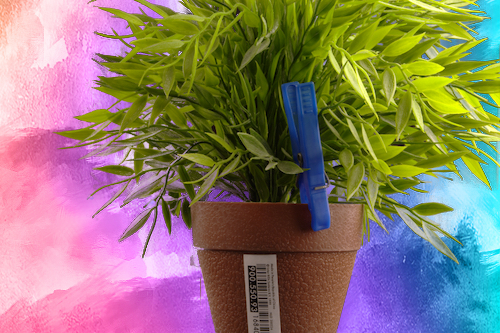
\includegraphics[width=\textwidth]{result1.png}
        \caption{Replacement}
    \end{minipage}
\end{figure}

\pagebreak

\section{OpenCV}

\begin{wrapfigure}{r}{4cm}
    
\includegraphics[width=4cm]{opencvlogo.png}
\end{wrapfigure}

OpenCV\cite{opencv} is a library
for computer vision. It contains a large
amount of tools, from GUIs, video analysis, machine learning,
object detection, image processing and many more\cite{opencvdoc}.
The library also contains a module about \textit{alpha matting},
which contains a function to generate alpha mattes given a trimap
\cite{opencvalphamatting}.

\subsection{Trimap colors}

As stated in the last section, the gray color represents the unknown pixels.
The library however, accepts a greyscale trimap.
The question is wheter different grays have different meanings.
This is not documented and would require to read the original
paper of implementation. \\ % cite
In order to find out here are a bunch of samples with different gray
colors:

\wrapfill

\begin{figure*}[h]
\makebox[\linewidth][c]{%
\centering
\subfigure[Trimap 1]{%
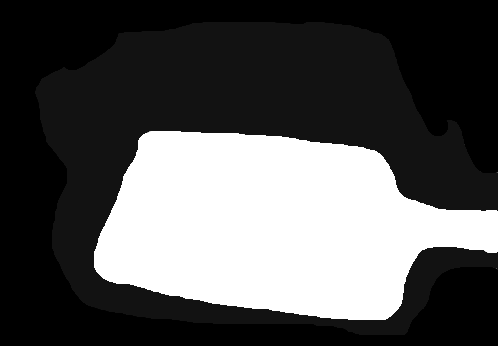
\includegraphics[width=0.25\textwidth]{brushes/trimap1.png}}%
\subfigure[Trimap 2]{%
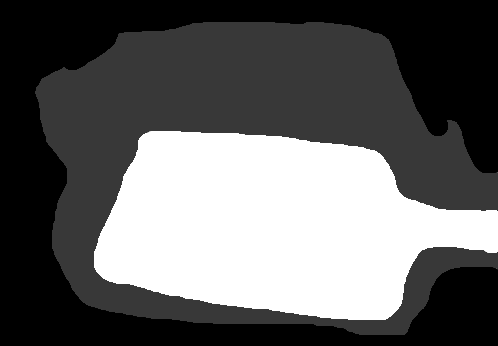
\includegraphics[width=0.25\textwidth]{brushes/trimap2.png}}%
\subfigure[Trimap 3]{%
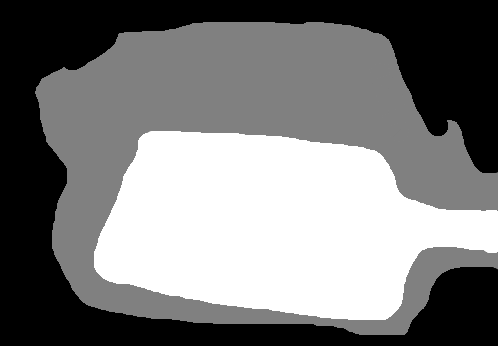
\includegraphics[width=0.25\textwidth]{brushes/trimap3.png}}%
\subfigure[Trimap 4]{%
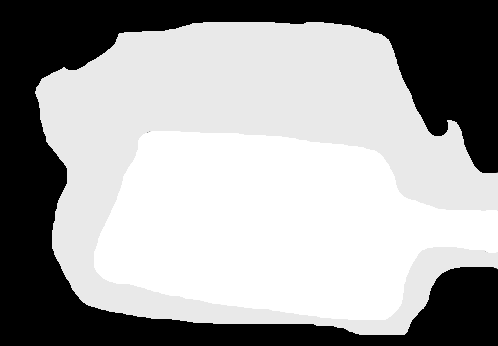
\includegraphics[width=0.25\textwidth]{brushes/trimap4.png}}%
}
\caption{Hairy brush trimaps}
\end{figure*}

\begin{figure*}[h]
\makebox[\linewidth][c]{%
\centering
\subfigure[Mask 1]{\label{fig:mask1}%
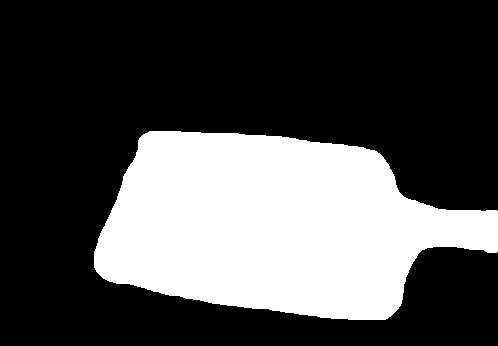
\includegraphics[width=0.25\textwidth]{brushes/mask1.png}}%
\subfigure[Mask 2]{\label{fig:mask2}%
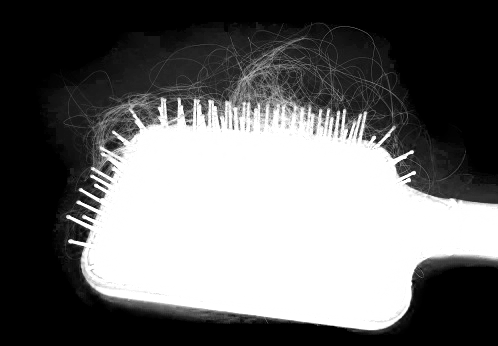
\includegraphics[width=0.25\textwidth]{brushes/mask2.png}}%
\subfigure[Mask 3]{\label{fig:mask3}%
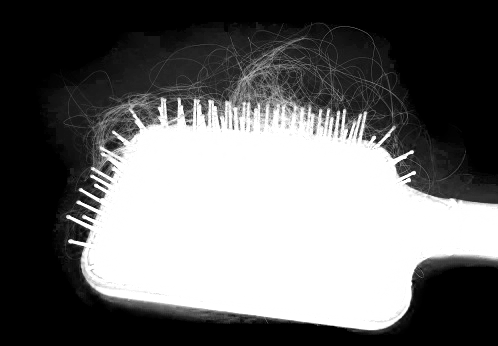
\includegraphics[width=0.25\textwidth]{brushes/mask3.png}}%
\subfigure[Mask 4]{\label{fig:mask4}%
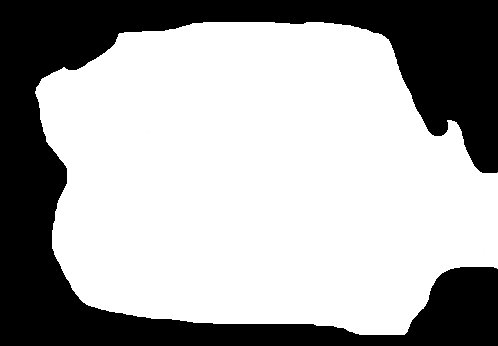
\includegraphics[width=0.25\textwidth]{brushes/mask4.png}}%
}
\caption{Hairy brush masks}
\end{figure*}
%
\begin{wrapfigure}{l}{7cm}
    \vspace{-\intextsep}
    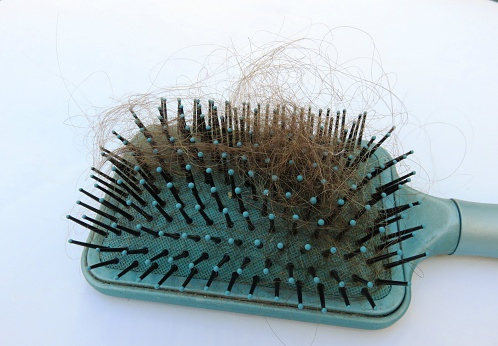
\includegraphics[width=7cm]{brushes/brush.jpg}
    \caption{Hairy brush}
\end{wrapfigure}

Given that this is the original image, we can confidently
infer that different gray values have the same meaning.
However, there is a range according to which a color is considered
\texttt{black}, \texttt{gray} or \texttt{white}.
As we can see in \ref{fig:mask1} and \ref{fig:mask4},
the unknown pixels have been considered to be background
or foreground respectively, because the gray value was too
low or too high.

\wrapfill

\pagebreak

\section{Implementation}

\subsection{OpenCV fundamental types}

The fundamental OpenCV type used in this project is the
\textbf{Mat}\cite{mat} type. A mat is essentially an
\(n\)-dimensional array. It can represent tensors, vector fields,
matrices and much more, both with real numbers or complex numbers.
For the purpose of this project, any mat represents a grayscale
or a colored image.

\subsection{OpenCV Binding}

The OpenCV library is primarily written in C++.
In order to access its functions in Rust, I used a crate
called \texttt{opencv}\cite{rustopencv}, which is a binding
to the \gls{FFI} of opencv.

It does not fully implement the Rust idioms and best pratices,
I found it very easy to accidentally cause a core dump
whilst calling a function.

The \textit{Flow Alpha Matting} module was developed by Muskaan Kularia
at Google Summer of Code 2019.

The code of interest is in the \texttt{opencv::alphamat} module,
and it contains the following function which computes alpha mattes of an object in an image.

\begin{lstlisting}[style=Rust, style=boxed]
    pub fn into_flow(
        image: &dyn ToInputArray,
        tmap: &dyn ToInputArray,
        result: &dyn ToOutputArray,
    ) -> Result<()>
\end{lstlisting}

\paragraph{Parameters:}
\begin{itemize}
    \item \textbf{image:} Input RGB image
    \item \textbf{tmap:} Input greyscale trimap image
    \item \textbf{result:} Output alpha matte image
\end{itemize}

The function intoFlow performs alpha matting on a RGB image
using a greyscale trimap image, and outputs a greyscale alpha matte image. \\
The output alpha matte can be used to softly extract the foreground
object from a background image. % cite

The \gls{trait}s \texttt{ToInputArray} and \texttt{ToOutputArray}
are implemented by the \texttt{Mat} type.

\pagebreak

\subsection{API Routes}

The routes are the following.
Note that each of them must include
a \texttt{multipart/form-data} attribute.

\begin{itemize}
    \item \textbf{POST}: \textbf{/api/matting} \\
        This endpoint returns in image representing the alpha mattes mask. \\
        The caller must specify two images: \textbf{target} and \textbf{trimap}.
    \item \textbf{POST}: \textbf{/api/fill/<color>} \\
        This endpoint replaces the background with a given color. \\
        The caller must specify two images: \textbf{target} and \textbf{mask}.
    \item \textbf{POST}: \textbf{/api/transparent} \\
        This endpoint removes the background and leaves it transparent. \\
        The caller must specify two images: \textbf{target} and \textbf{mask}.
    \item \textbf{POST}: \textbf{/api/replace} \\
        This endpoint replaces the background with a given image. \\
        The caller must specify three images: \textbf{target}, \textbf{mask} and \textbf{replacement}.
\end{itemize}

\subsection{Matting library}

The core of this project is certinaly the alpha matting algorithm.
In order to develope both a CLI and a GUI tool to
use this algorithm, I created a separate library (\texttt{matting-lib})
containing all the matting and image processing related functions.

The library exports the following functions, modules and structures

\begin{lstlisting}[style=Rust, style=boxed]
pub use image::{ImageFormat, DynamicImage};
pub use opencv::imgcodecs::*;

/// Export error module
pub mod error;

pub fn generate_mask(target: &Mat, trimap: &Mat) -> MessageResult<Mat>

pub fn same_size<P: AsRef<Path>>(path1: P, path2: P) -> MessageResult<bool>

pub fn bytes_to_mat(data: &[u8], flags: i32) -> MessageResult<Mat>

pub fn read_as_mat(filename: &str, flags: i32) -> MessageResult<Mat>

pub fn read_as_image(filename: &str) -> MessageResult<DynamicImage>

pub fn bytes_to_image(data: &[u8]) -> MessageResult<DynamicImage>

pub fn mat_to_dynamic_image_gray(mat: &Mat) -> MessageResult<DynamicImage>

pub fn remove_background(image: &RgbImage, mask: &RgbImage) -> DynamicImage

pub fn replace_background(
    image: &RgbImage,
    mask: &RgbImage,
    replacement: &RgbImage,
) -> DynamicImage

pub fn fill_background(
    image: &RgbImage,
    mask: &RgbImage,
    color: [u8; 4],
) -> DynamicImage

pub fn image_to_format(image: DynamicImage, format: ImageFormat) -> Vec<u8>
\end{lstlisting}

The \texttt{error} module exports error management utils

\begin{lstlisting}[style=Rust, style=boxed]
#[derive(Debug)]
pub struct MessageError {
    pub message: String,
}

impl MessageError {
    pub fn new(message: String) -> Self;
}

/// Result type
pub type MessageResult<T> = Result<T, MessageError>;


/// Conversion traits implementation

impl From<String> for MessageError;

impl From<&str> for MessageError;

impl From<OpencvError> for MessageError;

impl From<ImageError> for MessageError;
\end{lstlisting}

\subsection{Website}

List of website features

The images uploaded cannot be bigger than 2MiB

If a transformation is applies whilst the mask is loading,
the site will wait until the mask is ready.

The trimap panting tool aren't enabled until an image is uploaded

The mask download button and the transformation
selector aren't enabled until a mask has been generated or uploaded.

The website will check wheter the image and the mask are of the same size

The website will check wheter the image, mask and replacement image are of the same size

The website will handle error responses from the server with an alert message

The header dropdown is responsive and needs to be toggled when the page
is small.

While drawing you can press ctrl+z to undo

\pagebreak

\subsubsection{Painting mechanics}

The painting is done via the Canvas API \cite{canvasapi}.

\subsubsection{Flood fill}

The flood fill algorithm is a simple implementation with a stack data structure.

\algnewcommand\And{\textbf{ and }}
\algnewcommand\Or{\textbf{ or }}

\begin{algorithm}
    \begin{algorithmic}
        \caption{Flood Fill}

        \State{\textbf{Input:} The pixel grid \texttt{pixels}, the fill color \texttt{fill}, the clicked pixel \texttt{clicked}}
        \State{\textbf{Output:} The processed pixels}

        \If{\(\text{clicked}_\text{color} = \text{fill}\)}
            \State{return}
        \EndIf{}
        \State{\(\text{stack} \gets []\)}
        \While{\(\neg\)stack.empty()}
            \State{\(\text{point} \gets \text{stack.pop()}\)}

            \If{\(\text{point}_x < 0 \Or \text{point}_y < 0 \Or \text{point}_x \geq \text{pixels}_\text{width} \Or \text{point}_y \geq \text{pixels}_\text{height}\)}
                \State{continue}
            \EndIf{}

            \If{\(\text{point}_\text{color} \neq \text{clicked}_\text{color} \)}
                \State{continue}
            \EndIf{}

            \State{\(\text{pixels}_{x,y} \gets \text{fill}\)}

            \State{\(\text{stack.push(} \{x: \text{point}_x+1, y: \text{point}_y\} \text{)}\)}
            \State{\(\text{stack.push(} \{x: \text{point}_x-1, y: \text{point}_y\} \text{)}\)}
            \State{\(\text{stack.push(} \{x: \text{point}_x, y: \text{point}_y+1\} \text{)}\)}
            \State{\(\text{stack.push(} \{x: \text{point}_x, y: \text{point}_y-1\} \text{)}\)}
        \EndWhile{}
    \end{algorithmic}
\end{algorithm}

\subsubsection{Undo feature}

Everything drawn onto the canvas, meaning each line and fill operations
are stored in a stack data structure.

\pagebreak

\listoffigures

\pagebreak

\nocite{*} % cite all entries

\printbibliography

\pagebreak

\printnoidxglossary

\end{document}

% TO USE
%
%
%
%

\begin{lstlisting}[style=Rust, style=boxed]
    let output = log!(
        "Generating soft mask",
        args.verbose,
        matting::generate_mask(&target, &trimap)? // heavy lifting
    );
\end{lstlisting}

\begin{lstlisting}[style=HTML, style=boxed]
    <div>
        <h1>Title</h1>
    </div>
\end{lstlisting}

\begin{lstlisting}[style=JS, style=boxed]
    function ciao() {
        console.log("ee");
    }
\end{lstlisting}

\begin{lstlisting}[style=TOML, style=boxed]
    # asd
    hello = "valore"
\end{lstlisting}

\begin{lstlisting}[style=nginx, style=boxed]
    server {
        server_name = _;
    }
\end{lstlisting}